\section{RL Framework}
After the Background Research, the planned framework to use was OpenAI's Spinning Up framework. They provide clean implementations of modern RL algorithms, and a basic interface to apply the algorithms to OpenAI Gym environments, then plot the results. However, OpenAI Spinning Up has some downsides and lack some important features that would be helpful during this project.

\subsection{RL Algorithm Implementation Differences} \label{RLF:imp-diff}
Spinning Up's main focus is education. Therefore the algorithm implementations are stripped down from the proposed versions from the original papers, so the algorithms would be easier to read and understand. Although this is good for education, the resulting algorithms do not perform up to their potential due to their simplicity. The performance of SAC which is the algorithm of choice for this project, used on different Gym environments can be seen in Figure \ref{fig:spinup-SAC}.

\begin{figure}[h]
     \centering
     \begin{subfigure}[b]{0.49\textwidth}
         \centering
         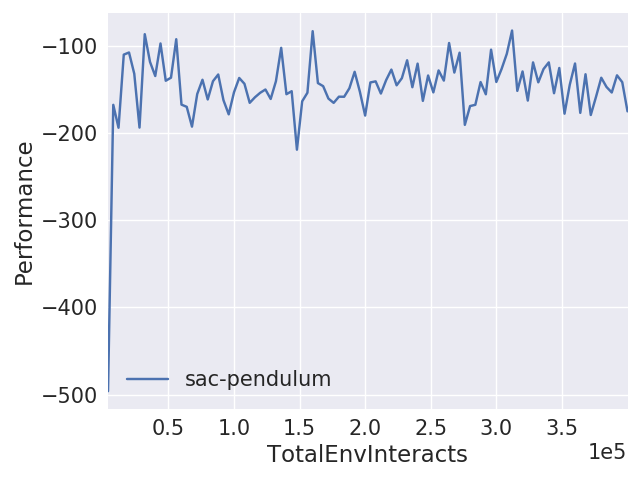
\includegraphics[width=\textwidth]{figures/rl-framework/sac-pendulum.png}
         \caption{Pendulum-v0 (Very Easy)}
     \end{subfigure}
     \hfill
     \begin{subfigure}[b]{0.49\textwidth}
         \centering
         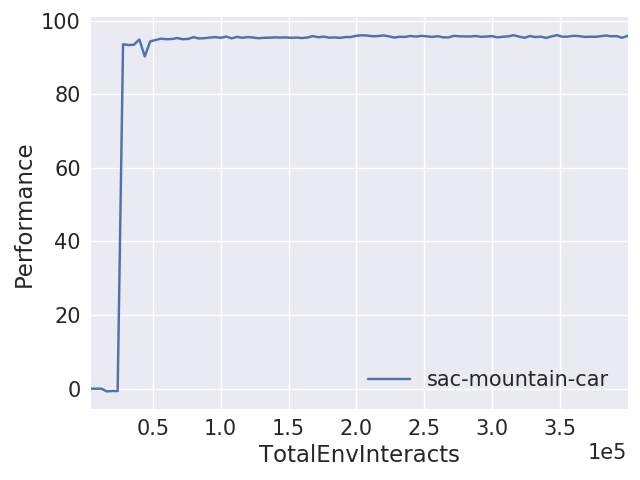
\includegraphics[width=\textwidth]{figures/rl-framework/sac-mountain-car.png}
         \caption{MountainCarContinuous-v0 (Easy)}
     \end{subfigure}
     \hfill
     \begin{subfigure}[b]{0.49\textwidth}
         \centering
         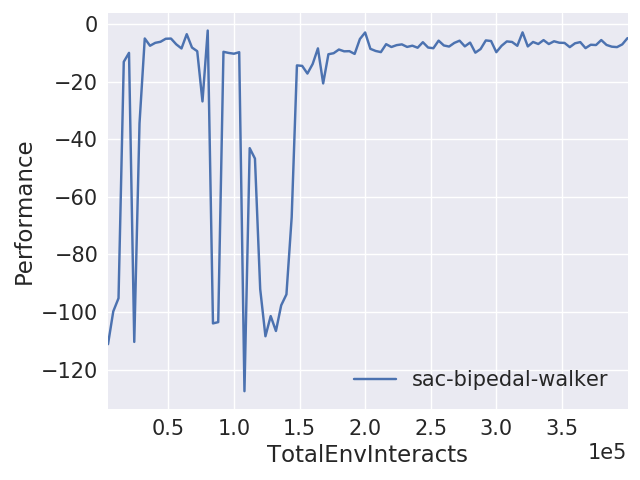
\includegraphics[width=\textwidth]{figures/rl-framework/sac-bipedal-walker.png}
         \caption{BipedalWalker-v3 (Hard)}
     \end{subfigure}
        \caption{Performance of Spinning Up implementation of SAC on different environments, using default parameters}
        \label{fig:spinup-SAC}
\end{figure}

Spinning Up implementation performs well and converges quickly on easy environments, but it provides disappointing results on the harder BipedalWalker-v3 environment. SAC is expected to have better exploration and achieve better results on BipedalWalker-v3 environment before 300.000 environment interacts \cite{gym-leaderboard}. But it never managed to escape a local minimum for a long period of training time. Considering our sailing environment will be pretty complex, Spinning Up implementation of SAC is not suitable for use on this project.

\newpage

\subsection{RL Framework Features} \label{RLF:framework-features}

Spinning Up Framework lacks some important features for Reinforcement Learning. First, it does not support continuing training of a previously trained agents. This is problematic in a few ways: it costs precious time and resources to train agents from scratch every time, plus even if models are trained again from ground up, no two reinforcement learning runs will be identical because of the noise or stochasticity in the algorithms.

The second lacking feature is that there is no hyperparameter optimization support. Hyperparameters can cause huge difference in performance \cite{hyperparameter-ddpg}. A comparison of DDPG on Walker2d-v1 with random hyperparameters can be seen in Figure \ref{fig:hyperparameter-ddpg}. The best and worst performing hyperparameters have approximately 3-fold average reward difference after 1 million timesteps.

\begin{figure}[h]
\centering
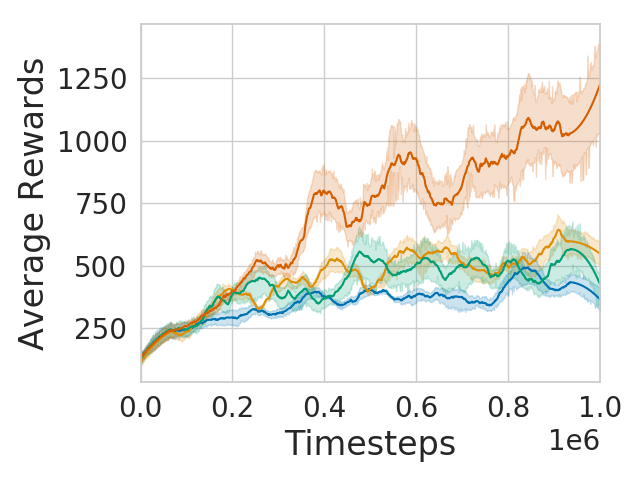
\includegraphics[width = 0.7\hsize]{figures/rl-framework/hyperparameter-ddpg.png}
\caption{Performance curve of DDPG on Walker2d-v1 with random hyperparameters \cite{hyperparameter-ddpg}}
\label{fig:hyperparameter-ddpg}
\end{figure}

Both of these features, and probably more that will arise during the course of this project are important for this project, So another framework with these features is needed.


\subsection{Stable Baselines 3}
Stable Baselines3 (SB3) is a library providing reliable implementations of state-of-the-art reinforcement learning algorithms in PyTorch, complete with a training framework 'RL Baselines3 Zoo' which contains scripts for training, evaluating agents, tuning hyperparameters, plotting results, and recording videos.\cite{stable-baselines3} 

SB3 solves both of the problems of Spinning Up Framework mentioned in sections \ref{RLF:imp-diff} and \ref{RLF:framework-features}. SB3 is focused on providing reliable implementations that can be used on Deep Reinforcement Learning Research, instead of the education focus of Spinning Up. SB3 implementations are fully functional, high quality, and they match the results of best previous implementations. Moreover, the RL Baselines Zoo has the missing features of Spinning Up's training framework, namely hyperparameter optimization and continuing training of previously trained models. Therefore, SB3 will be the choice of RL Framework for this project from now on.
